%!TEX root = thesis.tex

\chapter{Background}
\label{ch:Background}
This chapter introduces the theory behind the implemented method and the terminology used in this report.

The notation used in the report is as follows. Upper-case letters are used for random variables, e.g. $O_t$ for the random variable of observations at time $t$. Lower-case letters are used to indicate specific values of the corresponding random variable, e.g. $o_t$ represents a specific value of the random variable $O_t$.

\section{Formulation and Terminology of POMDPs}
A Markov decision process (MDP) is a mathematical framework for modeling sequential decision making problems and the framework forms the basis for the POMDP framework, which is a generalization of MDPs. In the MDP framework the state of the world is directly observable whereas in the POMDP framework it is only partially observable. When the state of the world cannot be determined directly a probability distribution over all the possible states of the world must be maintained. More detailed information about POMDPs can be found in \cite{Kaelbling1998} and \cite{Aberdeen2003}.

\subsection{The POMDP World Model}
\label{sec:POMDPModel}
The acting entity in the POMDP world model, the learner, is called an \emph{agent}. The world model in the POMDP framework consists of the following:

\begin{itemize}
  \item $\mathcal{S} = \{1, \dotsc, |\mathcal{S}|\}$ -- States of the world.
  \item $\mathcal{A} = \{1, \dotsc, |\mathcal{A}|\}$ -- Actions available to the agent.
  \item $\mathcal{O} = \{1, \dotsc, |\mathcal{O}|\}$ -- Observations the agent can make.
  \item Reward $r(i) \in \mathds{R}$ for each state $i \in \mathcal{S}$.
\end{itemize}
At time $t$, in state $S_t$, the agent takes an action $A_t$ according to its policy, makes an observation $O_t$, transitions to a new state $S_{t+1}$ and collects a reward $r(S_{t+1})$ according to the reward function $r(i)$. The state transition is made according to the system dynamics that are modeled by the transition model discussed in \ref{sec:TransitionModel}. Figure \ref{fig:POMDPModel} illustrates this along with the relations between MDPs and POMDPs.

\begin{figure}[ht]
  \centering
  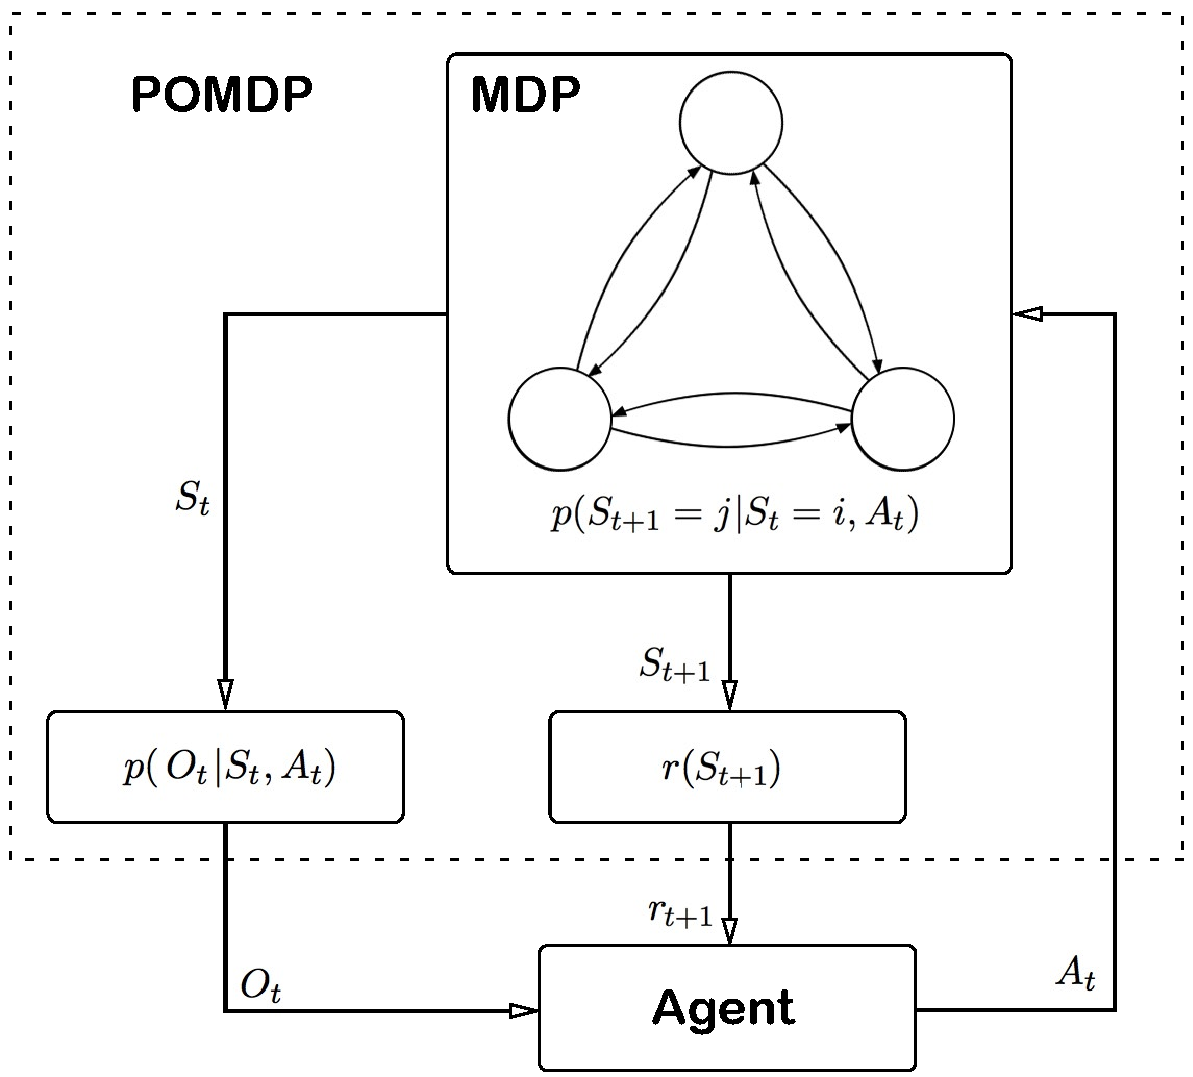
\includegraphics[width=0.5\textwidth]{figures/pomdp_model}
  \caption{POMDP diagram. In an MDP the agent would observe the state, $S_t$, directly. In POMDPs the agent makes an observation, $O_t$, that is mapped to the state $S_t$ by a stochastic process. Figure adapted from \cite{Aberdeen2003}.}
  \label{fig:POMDPModel}
\end{figure}

To put these concepts into context consider the problem of a robot that needs to find its way out of a maze. In the POMDP world model for that problem the robot is the agent and the state could be the location of the robot in the maze. The actions could be that the robot decides to move in a certain direction or even use one of its sensors. An observation could then be a reading from that sensor.

Since this example is easy to grasp it will be used throughout this report where deemed necessary.

\subsection{Transition Model}
\label{sec:TransitionModel}
The transition model defines the probabilities of moving from the current state to any other state of the world for any given action. For each state and action pair $(S_t = i, A_t = k)$ we write the probability of moving from state $i$ to state $j$ when action $A_t = k$ is taken as
\begin{equation}
  p(S_{t+1} = j|S_t = i, A_t = k)
\end{equation}
When a transition from state $i$ to state $j$ is for some reason impossible given action $k$, this probability is zero. An example of this would be when the agent takes an action that is intended to sense the environment and not move the agent. When the system dynamics prohibit all transitions, i.e. the state never changes, this probability is 1 for $i = j$ and zero otherwise, i.e.
\begin{equation}
\label{eq:IdentityTransitionModel}
  p(S_{t+1} = j|S_t = i, A_t = k) = 
  \begin{cases}
    1 & \text{if $i = j$}\\
    0 & \text{otherwise}
  \end{cases}
\end{equation}
The transition model for a specific problem is generally known or estimated using either empirical data or simply intuition.

\subsection{Belief States}
Because of the partial observability the agent is unable to determine its current state. However, the observations the agent makes depend on the underlying state so the agent can use the observations to estimate the current state. This estimation is called the agent's belief, or the belief state.
\begin{equation*}
  \mathcal{B} = \{1, \dotsc, |\mathcal{B}|\} \text{ -- Belief states, the agent's belief of the state of the world.}
\end{equation*}
A single belief state at time $t$, $B_t$, is a probability distribution over all states $i \in \mathcal{S}$. The probability of the state at time $t$ being equal to $i$, given all actions that have been taken and observations that have been made, is defined as
\begin{equation}
  B_t^i \defeq p(S_t = i | A_{1:t}, O_{1:t})
\end{equation}
Each time the agent takes an action and makes a new observation it gains more information about the state of the world. The most obvious way to keep track of this information is to store all actions and observations the agent makes, but that results in an unnecessary use of memory and computing power. It is possible to store all the acquired information within the belief state and update it only when necessary, after taking actions and making observations, without storing the whole history of actions and observations.

Given the belief state $b_t$, current action $a_t$ and observation $o_t$ the belief for state $j$ can be updated using
\begin{equation}
  \label{eq:UpdateBelief}
  b_t^j = \frac{ p(o_t | S_t = j, a_t) \sum_{i} p(S_t = j | S_{t-1} = i, a_t) b_{t-1}^i } { p(o_t) }
\end{equation}
If the state never changes we can simplify equation \eqref{eq:UpdateBelief} to

\begin{equation}
  \label{eq:UpdateBeliefFixedTarget}
  b_t^j = \frac{ p(o_t | S_t = j, a_t) b_{t-1}^j }{ p(o_t) }
\end{equation}
where $p(o_t)$ can be treated as a normalization factor. The derivations of \eqref{eq:UpdateBelief} and \eqref{eq:UpdateBeliefFixedTarget} are presented in Appendix \ref{app:BeliefUpdates}.

\subsection{Reward Function}
\label{sec:RewardFunction}
After each state transition the agent gets a reward according to the reward function. These rewards are the agent's indication of its performance and they are generally extrinsic and task-specific. In the case of a robot finding its way out of a maze the reward function might return a small negative reward for all states the robot visits and a large positive reward for the end state, i.e. when the robot is out of the maze, as described in \ref{sec:ModelBasedvsModelFree}. Since the goal is to find a policy that maximizes the expected total rewards the robot will learn to find the shortest path out of the maze.

The reward function may depend on the current action and either the current or the resulting state, but it can be made dependent on the resulting state only without loss of generality \cite{Aberdeen2003}. In Section \ref{sec:InformationRewards} we show how a reward function can be made dependent on the belief state only.

\subsection{Policy}
When it is time for the agent to act it consults its policy. The agent's policy is a mapping from states to actions that defines the agent's behavior. Finding a solution to a POMDP problem is done by finding the optimal policy, i.e. a policy that provides the optimal action for every state the agent visits, or approximating it when finding an exact solution is infeasible.

We already know that in POMDPs the agent is unable to determine its current state and a mapping from states to actions is therefore useless for the agent. The straightforward solution to this is to make the policy depend on the belief state. That is typically done by parameterizing the policy as a function of the belief state. Finding or approximating the optimal policy therefore becomes a search for the optimal policy parameters. 

\subsection{Logistic Policies}
\label{sec:LogisticPolicies}
One way of parameterizing a policy is to represent it as a function with policy parameters $\theta \in \mathds{R^{|\mathcal{A}| \times |\mathcal{S}|}}$, where $\mathcal{A}$ is the set of actions available to the agent and $\mathcal{S}$ the set of states of the world as presented in \ref{sec:POMDPModel}. Then $\theta$ forms a $|\mathcal{A}| \times |\mathcal{S}|$ matrix which in combination with the current belief state, $b_t$, forms a set of linear functions of the belief state. If $\theta^i$ represents the $i$th row of the matrix $\theta$ then we can select an action according to the policy with
\begin{equation}
  a_{t+1} = \argmax{i} \theta^i \cdot b_t
\end{equation}
This is a deterministic policy since it will always result in the same action for a particular belief state $b_t$. However, if we need a stochastic policy -- as is the case for the policy gradient method described in \ref{sec:GradientAscent} -- we can represent it as a logistic function using the policy parameters $\theta$ and the current belief state, $b_t$. Again, if $\theta^i$ represents the $i$th row of the matrix $\theta$ then the probability of taking action $k$ is given by
\begin{equation}
\label{eq:LogisticPolicy}
  p(A_{t+1} = k | b_t, \theta) = \frac{ \exp{(\theta^k \cdot b_t)} }{ \sum_{i=1}^{|\mathcal{A}|}{ \exp{( \theta^i \cdot b_t}) }} 
\end{equation} 
where $b_t$ is the agent's belief. This is a probability distribution that represents a stochastic policy. Taking an action based on this stochastic policy is done by sampling from the probability distribution.

The key to estimating the policy gradient in equation \eqref{eq:PolicyGradient} lies in calculating the gradient of equation \eqref{eq:LogisticPolicy} with respect to $\theta$, as shown in \cite{Butko2010b}.

\subsection{Observation Model}
\label{sec:ObservationModel}
When training a policy, the agent must be able to make observations. The sensors the agent uses to observe the world are in general imperfect and noisy which means that when the agent makes an observation it has to assume some uncertainty.

The observations available to the agent can be actual readings from its sensors -- and that is the case when the agent is put to work in the real world -- but during training, having a model that can generate observations is preferred. This is called an observation model and its purpose is to model the noisy behavior of the actual sensors.

The observation model needs to be estimated or trained using real data acquired by the agent's sensors before training the policy.

\subsection{Observation Likelihood}
\label{sec:ObservationLikelihood}
The observation likelihood is the probability of making observation $O_t$ after the agent takes action $A_t$ in state $S_{t}$,
\begin{equation}
  p(O_t|S_t, A_t)
\end{equation}
given the current observation model.

\subsection{Model-based vs. Model-free}
\label{sec:ModelBasedvsModelFree}
When the observation model, the transition model and the reward function $r(i)$ are all known, the POMDP is considered to be \emph{model-based}. Otherwise the POMDP is said to be \emph{model-free}.

A model-free POMDP can learn a policy without a full model of the world by sampling trajectories through the state space, either by interacting with the world or using a simulator. To give an example, consider our robot friend again that needs to find its way out of a maze. If the robot receives a small negative reward in each state it visits and a large positive reward when it gets out, it can learn a policy by exploring the maze without necessarily knowing the transition model or observation model.

The POMDPs considered in this report are always model-based.

\section{Policy Gradient}
\label{sec:PolicyGradient}
Methods for finding exact optimal solutions to POMDPs exist but they become infeasible for problems with large state- and action-spaces and they require full knowledge of the system dynamics, such as the transition model and the reward function. When either of those requirements are not fulfilled, reinforcement learning can be used to estimate the optimal policy.

The methods used, when exact methods are infeasible, are either value function methods or direct policy search. Value function methods require the agent to assign a value to each state and action pair and this value represents the long term expected reward for taking an action in a given state. In every state the agent chooses the action that has the highest value given the state, so the policy is essentially extracted from the value function. As the state-space grows larger the value function becomes more complex, making it more challenging to learn. However, the policy-space does not necessarily become more complex, making it more desirable to search the policy-space directly \cite{Aberdeen2003}. 

An algorithm for a direct policy search using gradient ascent was presented in \cite{BaxterB2001} and used in \cite{Butko2010b}. The algorithm generates an estimate of the gradient of the average reward with respect to the policy and using gradient ascent the policy is improved iteratively. This requires a parameterized representation of the policy.

\subsection{Gradient Ascent}
\label{sec:GradientAscent}
If the policy is parameterized by $\theta$, for example as described in \ref{sec:LogisticPolicies}, the average reward of the policy can be written as 
\begin{equation}
  \underbrace{\eta(\theta)}_{\mathclap{\substack{\text{Average} \\ \text{reward}}}} = \sum_{x \in X} \underbrace{r(x)}_{\text{reward}} \overbrace{p(x | \theta)}^{\substack{\text{prob. of $x$} \\ \text{given policy}}} = \Ex [r(x)]
\end{equation}
where $x$ represents the parameters that the reward function depends on. In our case $x$ is the agent's belief, $b$. The gradient of the average reward given the parameterized policy $\theta$ is therefore
\begin{align}
  \nabla \eta(\theta) &= \sum_{b \in \mathcal{B}} r(b) \nabla p(b | \theta) \\
                      &= \sum_{b \in \mathcal{B}} r(b) \frac{\nabla p(b | \theta)}{p(b | \theta)} p(b | \theta) \\
                      &= \Ex \bigg{[}r(b) \frac{\nabla p(b | \theta)}{p(b | \theta)}\bigg{]}
\end{align}
If we generate $N$ i.i.d. samples from $p(b | \theta)$ then we can estimate $\nabla \eta(\theta)$ by
\begin{equation}
  \widetilde{\nabla} \eta(\theta) = \frac{1}{N} \sum_{i=1}^N r(b_i) \frac{\nabla p(b_i | \theta)}{p(b_i | \theta)}
  \Bigg{\}} \substack{\text{given fixed $\theta$} \\ \text{we sample $b_i$} \\ \text{and we estimate} \\ \text{$\nabla \eta(\theta)$}}
\end{equation}
with $N \to \infty$, $\widetilde{\nabla} \eta(\theta) \to \nabla \eta(\theta)$.
\\\\
Assume a regenerative process, each i.i.d. $b_i$ is now a sequence $b_i^1 \dotsc b_i^{M_i}$.
We get
\begin{equation}
  \widetilde{\nabla} \eta(\theta) = \frac{1}{N} \sum_{i=1}^N r(b_i^1, \dotsc, b_i^{M_i}) \sum_{j=1}^{M_i} \frac{\nabla p(b_i^j | \theta)}{p(b_i^j | \theta)}
\end{equation}
If we assume
\begin{equation}
  r(b_i^1, \dotsc, b_i^{M_i}) = f\Big{(} \underbrace{r(b_i^1, \dotsc, b_i^{M_{i-1}})}_{r_i^{M_{i-1}}}, b_i^{M_i}\Big{)}
\end{equation}
and write
\begin{equation}
  \sum_{j=1}^{M_i} \frac{\nabla p(b_i^j | \theta)}{p(b_i^j | \theta)} = Z_i^{M_i} = Z_i^{M_{i-1}}  + \frac{\nabla p(b_i^{M_i} | \theta)}{p(b_i^{M_i} | \theta)}
\end{equation}
we have
\begin{equation}
  \widetilde{\nabla} \eta(\theta) = \frac{1}{N} \sum_{i=1}^N \underbrace{r_i^{M_i} Z_i^{M_i}}_{\substack{\text{Computed} \\ \text{iteratively}}} \bigg{\}} \frac{1}{N} \widetilde{\nabla}_N
\end{equation}
where
\begin{equation}
  r_i^{M_{i}} = r(b_i^1, \dotsc, b_i^{M_i})
\end{equation}
This gives an unbiased estimate of the policy gradient
\begin{equation}
  \label{eq:GradientEstimate}
  \underbrace{\widetilde{\nabla}_N}_{\substack{\text{Computed} \\ \text{iteratively}}} = \widetilde{\nabla}_{N-1} + r_N^{M_N} Z_N^{M_N}
\end{equation}
The estimate of the gradient of the average reward, $\widetilde{\nabla}_N$, can therefore be computed iteratively and the policy parameters $\theta$ updated by a simple update rule 
\begin{equation}
\label{eq:PolicyGradient}
  \theta_{new} = \theta + \frac{\widetilde{\nabla}_N}{N}
\end{equation}
where $N$ is the number of samples used to estimate the gradient, i.e. the number of episodes.

When training a policy using gradient ascent the gradient of the average reward is estimated from a number of episodes, during which the policy parameters are kept fixed. When all episodes have finished the policy parameters are updated using the gradient estimation and that concludes one training iteration, a so called epoch.

The gradient estimate is what has been referred to as the policy gradient.

\section{Infomax Control}
Using the theory of optimal control in combination with information maximization is known as \emph{Infomax control} \cite{Movellan2005}. The idea is to treat the task of learning as a control problem where the goal is to derive a policy that seeks to maximize information, or equivalently, reduce the total uncertainty. The POMDP models that are used for this purpose are information gathering POMDPs and have been called Infomax POMDPs, or I-POMDPs \cite{Butko2010b}.

\section{Information Rewards}
\label{sec:InformationRewards}
Conceptually, the POMDP world issues rewards to the agent as it interacts with the world and these rewards are generally task-specific. In order to make an information-driven POMDP, an I-POMDP, the reward function must depend on the amount of information the agent gathers. The way this is done is to make the reward a function of the agent's belief of the world. The entropy of the agent's belief at each point in time becomes the reward the agent receives. As the agent becomes more and more certain about the state of the world, the higher reward the agent receives. This principle is what drives the learning of information gathering strategies. The policy gradient is used to adjust the current policy and the reward, i.e. the certainty of the agent's belief, controls the magnitude of the adjustment. This is shown in equation \eqref{eq:GradientEstimate}.

The information reward function becomes
\begin{equation}
\label{eq:InformationRewards}
  r_t(b_t) = \sum_{j=1}^{|\mathcal{S}|} b_t^j \log_2{b_t^j}
\end{equation}
where $\mathcal{S}$ is the set of states of the world and $b_t$ is the agent's belief at time $t$.

Care needs to be taken when calculating the logarithm of the belief in practice because as the agent becomes more certain about the state of the world, most of the values of the belief vector $b_t$ approach zero. As the precision of numbers stored in computers varies, we might have the situation where some of those values are actually stored as zero. Therefore, when calculating the rewards we define

\begin{equation}
  \log_2{0} \defeq 0
\end{equation}
